\documentclass{article}
\usepackage{amsmath}

% Define \argmax command
\DeclareMathOperator*{\argmax}{arg\,max}
\usepackage{amssymb}
\usepackage{graphicx}
\usepackage{float}
\usepackage{enumitem}
\usepackage{forest}

\begin{document}

\title{Homework 3}
\author{Manyara Bonface Baraka - mbaraka}
\date{\today}
\maketitle

\section*{Problem 1: Value Iteration for Markov Decision Processes}
Value iteration is a dynamic programming aligorithm tha tis used to fid the optimal value function and policy for a markov decision process.

\subsection*{Understanid MDPs}
MDP is defined by:
\begin{itemize}
    \item \textbf{State (S)} possible configurations of the environment
    \item \textbf{Actions (A)} possible decisions or moves the agent can make
    \item \textbf{Transition Model (T)} probability of moving from one state to another given an action
    \item \textbf{Reward Function (R)} immediate reward received after transitioning from one state to another
    \item \textbf{Policy (\(\pi\))} mapping from states to actions that defines the agent's behavior
\end{itemize}

\subsection*{Value funcion and policy that results:}
\subsubsection*{Optimal Value Function and Policy:}

The optimal value function and policy obtained from the value iteration algorithm are as follows:

\paragraph{Optimal Value Function:}
\[
\begin{bmatrix}
0.0689 & 0.0614 & 0.0744 & 0.0558 \\
0.0919 & 0.0000 & 0.1122 & 0.0000 \\
0.1454 & 0.2475 & 0.2996 & 0.0000 \\
0.0000 & 0.3799 & 0.6390 & 0.0000
\end{bmatrix}
\]

\paragraph{Optimal Policy:}
\[
\begin{bmatrix}
0 & 3 & 0 & 3 \\
0 & 0 & 0 & 0 \\
3 & 1 & 0 & 0 \\
0 & 2 & 1 & 0
\end{bmatrix}
\]

\paragraph{Episode Outcome:}
The episode finished with a reward of \(1.0\).
\clearpage

\section*{Problem 2: SARSA for Markov Decision Processes}

SARSA(State-Action-Reward-State-Action) is an on-policy reignforcement learning alifgorithm used to lean the optimal policy for an MDP without
knowing transition probabilities. Unlike value iteration which is a dynamic programming method requiring a known transition model, SARSA is am odel-free Learning aligorithm taht learns from direct experiment.

\subsection*{Understanding SARSA}
SARSA is defined by the following key components:

\begin{itemize}
    \item \textbf{State (\(S\))}: The current configuration of the environment.
    \item \textbf{Action (\(A\))}: The decision or move the agent takes in a given state.
    \item \textbf{Reward (\(R\))}: The immediate feedback received after taking an action in a state.
    \item \textbf{Next State (\(S'\))}: The state the agent transitions to after taking an action.
    \item \textbf{Next Action (\(A'\))}: The action the agent plans to take in the next state.
\end{itemize}

The SARSA algorithm updates the Q-value (state-action value) using the following equation:

\[
Q(S, A) \leftarrow Q(S, A) + \alpha \left[ R + \gamma Q(S', A') - Q(S, A) \right]
\]

where:
\begin{itemize}
    \item \(Q(S, A)\): The current estimate of the Q-value for state \(S\) and action \(A\).
    \item \(\alpha\): The learning rate, which determines how much new information overrides old information.
    \item \(\gamma\): The discount factor, which determines the importance of future rewards.
    \item \(R\): The reward received after taking action \(A\) in state \(S\).
    \item \(Q(S', A')\): The Q-value of the next state-action pair.
\end{itemize}

SARSA is called an on-policy algorithm because it updates the Q-value based on the action \(A'\) that the agent actually takes, following its current policy.

\subsection*{Comparizon of SARSA vs Value Iteration}
\begin{itemize}
    \item \textbf{Value Iteration:}
    \begin{itemize}
        \item Requires a known transition model and reward function.
        \item Computes the optimal value function and policy by iteratively updating the value of each state.
        \item Guarantees convergence to the optimal policy for MDPs.
        \item Computationally expensive for large state spaces.
    \end{itemize}
    \item \textbf{SARSA:}
    \begin{itemize}
        \item Does not require a known transition model; learns from direct interaction with the environment.
        \item Updates the Q-value based on the current policy, making it an on-policy algorithm.
        \item Can adapt to changes in the environment during learning.
        \item May converge to a suboptimal policy if the exploration strategy is not well-designed.
    \end{itemize}
\end{itemize}

\subsection*{Value funcion and policy that results:}

\paragraph{SARSA Optimal Value Function:}
\[
\begin{bmatrix}
0.068 & 0.111 & 0.209 & 0.098 \\
0.063 & 0.000 & 0.373 & 0.000 \\
0.082 & 0.197 & 0.412 & 0.000 \\
0.000 & 0.317 & 0.643 & 0.000
\end{bmatrix}
\]

\paragraph{SARSA Optimal Policy:}
\[
\begin{bmatrix}
1 & 3 & 3 & 3 \\
0 & 0 & 0 & 0 \\
3 & 1 & 0 & 0 \\
0 & 2 & 2 & 0
\end{bmatrix}
\]

\subsection*{Why use SARSA instead of Value Iteration}

\subsection*{Differences:}

\begin{itemize}
    \item \textbf{Policy:} SARSA's policy differs slightly due to exploration (\(\epsilon = 0.1\)), leading to safer paths avoiding holes while for 
    Value Iteration's policy is deterministic and model-based.
    \item \textbf{Value Function:} SARSA's values are estimates based on experience, which are lower due to exploration while for 
    Value Iteration it provides exact values using known transitions.
\end{itemize}

\subsection*{Why Use SARSA?}

SARSA is model-free, making it suitable for environments where transition probabilities are unknown. 
It learns through interaction, essential for real-world applications without a known model.
 Value Iteration requires full knowledge of the environment's dynamics, which is often unavailable.



\clearpage
\section*{Problem 3: Bayesian Network}
Bayesian network is the probabilistic graphical model that represents set of random vaiable and their Conditional
independecies using the Directed Acyclic Graph. It helps in reasoning under uncertaninty by usind Bayes Theorom.\\
Each node of the BN represent a random vvaiable  and directed edges between nodes represent casual dependecies. The Conditional probablity
Tables(CPT) are used to quanityfy the relationships.

\subsubsection*{BNS Structure for this problem}
Since BN representsvariable as nodes and dependecies as directe edges, Thereforer this problem:

\textbf{parent node:} Disease {flu or Step throst}
\textbf{Child NOdes:} Fever, Cough and sore throat that is the syptoms depend on the Disease


\begin{center}
\begin{forest}
for tree={
    grow=east,
    edge={-latex},
    parent anchor=east,
    child anchor=west,
    align=center,
    l sep=15mm
}
[Disease
    [Fever]
    [Cough]
    [Sore Throat]
]
\end{forest}
\end{center}


\subsubsection*{Conditional probablity Tables}
Each node has a Conditional Probability Table (CPT) that defines probabilities conditioned on its parents.\\
Assuming equal probabilities since no prior information is provided:
\[
P(\text{Flu}) = 0.5, \quad P(\text{Strep}) = 0.5
\]
The conditional probabilities of symptoms given the disease are as follows:

\begin{table}[H]
\centering
\begin{tabular}{|c|c|c|c|}
\hline
\textbf{Disease} & \textbf{P(Fever = Yes)} & \textbf{P(Cough = Yes)} & \textbf{P(Sore Throat = Yes)} \\ \hline
Flu              & 0.6                     & 0.5                     & 0.3                          \\ \hline
Strep            & 0.4                     & 0.8                     & 0.6                          \\ \hline
\end{tabular}
% \caption*{Conditional Probability Table for Symptoms}
\end{table}

\subsubsection*{How are the probabilities stored and how are they used for inference?}
The probabilities are stored in Conditional Probability Tables (CPTs) for each node in the Bayesian Network. 
Each CPT specifies the probability of a node given its parent(s). For example:

- \( P(\text{Fever} | \text{Disease}) \)
- \( P(\text{Cough} | \text{Disease}) \)
- \( P(\text{Sore Throat} | \text{Disease}) \)

These probabilities are used for inference by applying Bayes' theorem and the chain rule of probability.
 For example, to compute the probability of a disease given observed symptoms, we use:

\[
P(\text{Disease} | \text{Symptoms}) \propto P(\text{Symptoms} | \text{Disease}) P(\text{Disease})
\]

where \( P(\text{Symptoms} | \text{Disease}) \) is computed as the product of the conditional probabilities of individual symptoms given the disease:

\[
P(\text{Symptoms} | \text{Disease}) = P(\text{Fever} | \text{Disease}) \cdot P(\text{Cough} | \text{Disease}) \cdot P(\text{Sore Throat} | \text{Disease})
\]

This allows us to perform reasoning and make predictions based on the given Bayesian Network.

\subsubsection*{Output}
\begin{table}[H]
\centering
\begin{tabular}{|l|c|}
\hline
\textbf{Disease}        & \(\phi(\text{Disease})\) \\ \hline
Disease(Flu)            & 0.3333                   \\ \hline
Disease(Strep)          & 0.6667                   \\ \hline
\end{tabular}
% \caption*{Prior Probabilities of Diseases}
\end{table}
\clearpage


\section*{Problem 4: Bayesian Network}
Wil use BN for spam filtering because spam filtering is a classification problem where we determin whether an email is spam or not based on its content.
\subsubsection*{Why BN}
\begin{itemize}
    \item \textbf{probabilistic Reasoning:} BN allow reasoning under unccertanity this is useful becasue the spam words may not always appear in the same context.
    \item \textbf{Explainability:} BN clearly shows how different words contibute to the probability of the spam
    \item \textbf{Handling missing data:} BN can make prediction using avaibleable data to predict missing words
    \item \textbf{Incremental Learning:} BN updates their knowledge as new spam mails are encountered.
\end{itemize}

\subsubsection*{How Bayesian Network work for Spam filtering}
\subsubsection*{Graphical Representation of Bayesian Network for Spam Filtering}
The Bayesian Network for spam filtering can be represented as a directed acyclic graph (DAG), where:

- The parent nodes represent features of the email (e.g., presence of specific words, sender reputation, etc.).
- The child node represents the classification (Spam or Not Spam).

\begin{center}
\begin{forest}
for tree={
    grow=east,
    edge={-latex},
    parent anchor=east,
    child anchor=west,
    align=center,
    l sep=15mm
}
[Spam Classification
    [Word Features
        [Word1]
        [Word2]
        [Word3]
    ]
    [Sender Reputation]
    [Email Length]
]
\end{forest}
\end{center}

This graphical representation shows how different features contribute to the classification decision in the Bayesian Network.


\subsubsection*{How would you extend the concept of using keywords to get the essence of the next text for the document classification?}
\begin{itemize}
    \item \textbf{Latent Semantic Analysis (LSA):} Use LSA to reduce the dimensionality of the document-term matrix and extract latent topics.
     These topics can serve as features for classification.
    \item \textbf{Word Embeddings:} Utilize word embeddings such as Word2Vec, GloVe to represent words in a continuous vector space. 
    Aggregate these embeddings through by averagin or any other metric to represent the document.
    \item \textbf{Topic Modeling:} Apply topic modeling techniques like Latent Dirichlet Allocation (LDA) to identify the main topics in the text.
     The topic distribution will be used as features for classification.
    \item \textbf{TF-IDF Features:} Compute Term Frequency-Inverse Document Frequency (TF-IDF) scores for words in the document. 
    Afterwards the scores are used to to identify the most important words and classify the document based on their presence.
    \item \textbf{Neural Networks:} Train a neural network like RNN, Transformer among others to learn the semantic relationships between words and classify the document based on its content.
\end{itemize}

\subsubsection*{Can Bayesian Networks be used for document classification?}
Yes, Bayesian Networks can be used for document classification. Here's how:

\begin{itemize}
    \item \textbf{Feature Representation:} Represent the document features (e.g., word frequencies, presence of specific keywords, etc.) as nodes in the Bayesian Network.
    \item \textbf{Class Node:} Add a node representing the document class (e.g., categories like sports, politics, etc.).
    \item \textbf{Conditional Probabilities:} Define the conditional probability tables (CPTs) for each feature node given the class node. These probabilities can be learned from training data.
    \item \textbf{Inference:} Use the Bayesian Network to compute the posterior probability of each class given the observed features of a document. The class with the highest posterior probability is selected as the predicted class.
\end{itemize}

Bayesian Networks are particularly useful for document classification when the relationships between features and classes are complex and when reasoning under uncertainty is required.

\subsubsection*{Write a pseudo code}
\begin{verbatim}
# Pseudo code for Bayesian Network-based Spam Filtering

# Step 1: Define the Bayesian Network structure
# Nodes: Features (e.g., Word1, Word2, Sender Reputation, Email Length), 
Spam Classification
# Edges: Directed edges from features to Spam Classification

# Step 2: Initialize Conditional Probability Tables (CPTs)
# Example:
# P(Spam) = 0.4, P(Not Spam) = 0.6
# P(Word1 | Spam) = 0.8, P(Word1 | Not Spam) = 0.2
# P(Word2 | Spam) = 0.7, P(Word2 | Not Spam) = 0.3
# ...

# Step 3: Input email features
# Example: Email contains Word1 and Word2, Sender Reputation = High, Email Length = Short

# Step 4: Compute posterior probabilities using Bayes' theorem
# For each class (Spam, Not Spam):
# P(Class | Features) \propto P(Features | Class) * P(Class)
# P(Features | Class) = P(Word1 | Class) * P(Word2 | Class) * ... * P(Sender Reputation | Class) * P(Email Length | Class)

# Step 5: Normalize probabilities
# P(Class | Features) = P(Class | Features) / Sum(P(Class | Features) for all classes)

# Step 6: Classify email
# Predicted class = argmax(P(Class | Features))

# Step 7: Output classification result
# Example: Email is classified as Spam with probability 0.85
\end{verbatim}
\clearpage

\subsection*{Problem 5: Applications of Hidden Markov Models}

\subsubsection*{The Chosen Paper and Applications}
\textbf{Paper:} \textit{"A Tutorial on Hidden Markov Models and Selected Applications in Speech Recognition" by Lawrence R. Rabiner (1989)}\\
\textbf{Application:} Predicting the movement of endangered species using GPS sensor data.\\
\textbf{How HHMs are Used:}
\begin{itemize}
    \item \textbf{Hidden States:} The species’ location in one of 10 geographic regions.
    \item \textbf{Observed States:} Discretized sensor readings (e.g., GPS coordinates mapped to 5 zones).
    HMMs model the transition between regions (persistence or movement) and the likelihood of sensor data given the true location.
\end{itemize}

\subsubsection*{HMM Parameters}

\paragraph{Hidden States:}
10 regions: \(\{R_0, R_1, \ldots, R_9\}\).

\paragraph{Observed States:}
5 sensor outputs: \(\{O_0, O_1, \ldots, O_4\}\).

\paragraph{Transition Probabilities:}
Model persistence and adjacency:
\[
P(R_i \to R_j) =
\begin{cases} 
0.6 & \text{if } i = j, \\
0.2 & \text{if } j = (i \pm 1) \mod 10, \\
0 & \text{otherwise}.
\end{cases}
\]

\paragraph{Emission Probabilities:}
Each region \(R_i\) primarily emits \(O_{i \mod 5}\):
\[
P(O_k \mid R_i) =
\begin{cases} 
0.7 & \text{if } k = i \mod 5, \\
0.075 & \text{otherwise}.
\end{cases}
\]

\paragraph{Initial State Distribution:}
Uniform:
\[
P(R_i) = 0.1 \quad \text{for all } i.
\]


\subsubsection*{Results and interpretation}

\subsection*{Results and Explanation}

\paragraph{Output:}
The results output sequence ( [0, 1, 0, 3, 2, 0, 4, 1, 2, 3, 0, 1]), outputs the most likely region at each time step.

\paragraph{Interpretation:}
The forward-backward algorithm computes the posterior probability 
\[
P(\text{Region}_t \mid \text{Observations}_{1:T})
\]
by combining:

\begin{itemize}
    \item \textbf{Forward messages (\(\alpha\))}: Likelihood of observations up to \(t\) and being in region \(R_i\).
    \item \textbf{Backward messages (\(\beta\))}: Likelihood of future observations given \(R_i\).
\end{itemize}

The result smooths over the entire sequence, leveraging past and future data to infer intermediate states
. For example, if the sensor data is noisy, the algorithm corrects it by considering the species’ tendency to stay in adjacent regions.


\clearpage

\section*{Problem 6: Implementing a Simple Kalman Filter}
Kalman Filter is a rucurvsive Bayesian filter that provides the optimal estimate of the hidden state of a linear dynamical systemn in the presence of Gaussian noise.

\subsubsection*{Kalman Math fund.}

A linear dynamical system evolves in discrete time according to the following equations:

\subsubsection*{(A) State Equation (Process Model)}
\[
x_{k+1} = A x_k + w_k
\]
where:
\begin{itemize}
    \item \(x_k\) is the hidden state (e.g., position and velocity of a moving object).
    \item \(A\) is the state transition matrix, which determines how the state evolves.
    \item \(w_k\) is the process noise, assumed to be Gaussian with mean zero and covariance \(Q\):
    \[
    w_k \sim \mathcal{N}(0, Q)
    \]
\end{itemize}

\subsubsection*{(B) Measurement Equation (Observation Model)}
\[
z_k = H x_k + v_k
\]
where:
\begin{itemize}
    \item \(z_k\) is the observation (measurement) at time \(k\).
    \item \(H\) is the observation matrix, which maps the hidden state to the measurement space.
    \item \(v_k\) is the measurement noise, assumed to be Gaussian with mean zero and covariance \(R\):
    \[
    v_k \sim \mathcal{N}(0, R)
    \]
\end{itemize}

The goal of the Kalman Filter is to estimate \(x_k\), given the noisy measurements \(z_k\).

\subsection*{Questions before implimentation}
\begin{itemize}
    \item \textbf{What are the connenection between Kalman Filter and HMM?what are the similarites and most important differences}
    \begin{itemize}
        \item \textbf{Connection:} Both Kalman Filters and Hidden Markov Models (HMMs) are probabilistic models used for state estimation in dynamic systems. They share the following similarities and differences:
            \begin{itemize}
                \item \textbf{Similarities:}
                \begin{itemize}
                    \item Both are used for sequential data and involve hidden states.
                    \item Both rely on probabilistic reasoning and Bayesian inference.
                    \item Both use transition models to describe how states evolve over time.
                \end{itemize}
                \item \textbf{Differences:}
                \begin{itemize}
                    \item Kalman Filters assume linear dynamics and Gaussian noise, while HMMs can handle discrete states and non-Gaussian noise.
                    \item Kalman Filters provide continuous state estimates, whereas HMMs focus on discrete state sequences.
                    \item Kalman Filters are computationally efficient for linear systems, while HMMs require more complex algorithms like the Forward-Backward algorithm for inference.
                \end{itemize}
            \end{itemize}
    \end{itemize}
    \item \textbf{What is the goal of Kalman Filter}
    \begin{itemize}
       \item  The goal of the Kalman Filter is to estimate the hidden state \(x_k\) of a linear dynamical system at each time step \(k\), given noisy measurements \(z_k\). 
        This involves combining prior knowledge about the system's dynamics (process model) with the observed data (measurement model) to produce an optimal estimate of the state.
         The Kalman Filter achieves this by minimizing the mean squared error of the state estimate.
    \end{itemize}
\end{itemize}


\subsection*{Implimentation output}
\begin{figure}[H]
\centering
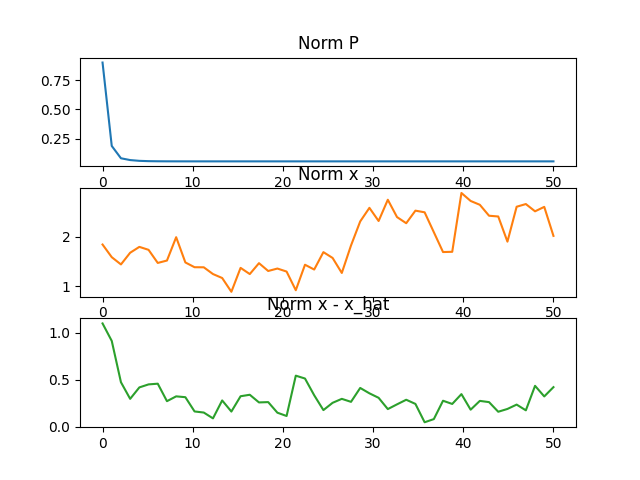
\includegraphics[width=1\textwidth]{Figure_kalman.png}
% \caption*{Illustration of the Kalman Filter Process}
\label{fig:kalman_filter}
\end{figure}


\subsection*{Questions after implimentation}
\begin{itemize}
    \item \textbf{Describe the significance/differences between the time update and measurement update.}
    \begin{itemize}
        \item \textbf{Time Update (Prediction Step):} This step predicts the state of the system at the next
         time step based on the current state estimate and the process model.
          It involves projecting the state and covariance forward in time. The time update is crucial
           for estimating the system's state before incorporating new measurements.

        \item \textbf{Measurement Update (Correction Step):} This step updates the predicted state using 
        the new measurement. It adjusts the state estimate and covariance based on 
        the difference between the predicted measurement and the actual measurement. 
        The measurement update ensures that the state estimate is corrected using the latest observed data.
    \end{itemize}
    \item \textbf{What is the significance of the measurement \(z\) having different dimensions to the signal vlues \(X\)}
    \begin{itemize}
        \item Measurements (\(z\)) often observe a subset or linear combination of the state (\(x\)). The matrix \(C\) maps the state to the measurement space, enabling partial observations.
    \end{itemize}
    \item \textbf{From the plot above, what can you say about shape of the curve \(P\) with respect to number of iteration? What does it show us about
    estimate of P and the Kalman Filter gain matrix \(K\)? In two sentences describe the meeningd of P and K matrices}
    \begin{itemize}
        \item \(P\) represents the covariance of the state estimate, which indicates the uncertainty in the estimate. 
        As the number of iterations increases, \(P\) typically decreases and seems to be stabilizing this indicastes convergence to the steady-state error covariance showing that the estimate becomes more certain over time.
        \item \(K\), the Kalman Gain, determines how much weight is given to the measurement versus the prediction. 
        As \(P\) decreases, \(K\) also decreases, indicating that the filter relies more on the prediction and less on the measurement. A stable \(P\) indicates an optimal \(K\).
    \end{itemize}
    \item \textbf{Proide the same analysis for the plot of the norm of x -x\_hat}
    \begin{itemize}
        \item The plot of the norm of \(x - \hat{x}\) typically shows a decreasing trend over iterations, indicating that the estimate \(\hat{x}\) is converging to the true state \(x\). This demonstrates the effectiveness of the Kalman Filter in reducing the estimation error over time. The norm of \(x - \hat{x}\) represents the magnitude of the estimation error, and its decrease signifies improved accuracy of the state estimate.
    \end{itemize}
    
\end{itemize}

\clearpage
\section*{Problem 7}
Predicting the sales of its product over the next year based on the historical sales data. 
\subsubsection*{Best Model to perform the task?}
\begin{enumerate}
    \item \textbf{Hidden Markov Models}
    \begin{itemize}
        \item Is a probabilisic model that assumes hiden states for sales levels such as low, medium orhigh and infere from the observed data such as advaerticememtn and pricing.
        \item It also has observations that measure variables like season, price and advertising spend.
        \item It also assumes the Markov propery that the current stat depends only on the previous state.
        \begin{itemize}
            \item However HMM cannot hanndle multiple dependecies, limited to the seasonal trend modeling and its only limited to one hidden variable
        \end{itemize}
    \end{itemize}
    

    \item \textbf{Dynamic Bayesian Network}
    \begin{itemize}
        \item Generalizes HMM by allowing more flexible dependecies and multi-variable state represntation insstead of a single hidden variable.
        \item Unlike HMM it can explicitly model the seasonal trends.
        \begin{itemize}
            \item Howver, its more complex and computationally expensive
        \end{itemize}
    \end{itemize}
    



    \item \textbf{Markov Decision Process}
    
    \begin{itemize}
        \item Its best in making decision on how much to spend on advertisin to maximize the future sales.
        \item It optimized the long term revenue also helps in deciding how much to invest in marketing, and accounts for uncertinity.
        \begin{itemize}
            \item However it requires defining awards which might be comples and computationally expensive for large state spaces.
        \end{itemize}
    \end{itemize}
    \item \textbf{Kalman Filter}
    \begin{itemize}
        \item Kalman Filter is best for real time tracking of the sales in the noisy sales.
        \item Its also computernally efficienen and can make real-time prediction.
        \begin{itemize}
            \item However,it assumes linear relationship and struggles with non-linear dependecies.
            \item It cannot model easily external variables like advertising.
        \end{itemize}
    \end{itemize}
\end{enumerate}

\subsubsection*{Best model fit to the task and why?}
Since sales are influenced by mulitple varibles and factors such as price, season, adverticing and others, DBN is the better choice as i allows modelling for multiple relationships.\\

\textbf{Why DBN is the best fit}
\begin{itemize}
    \item Multiple variable: DBN facotrs in and can easily model multiple varibles such as advertising, price and season that other Models cannont explicitly model.
    \item Long-term dependecies: DBN can model how external variables like advertising how it affects the sales over time.
    \item Better Accuracy: DBN captures the real-world dependecies.
\end{itemize}

\subsubsection*{Implimentation of DBN}
\begin{itemize}
    \item Defining the sales varibales: Sales, Adverts, Price and season
    \item Construct Bayesian Network at each time step
    \item Define the Conditional probablities.
    \item Use pomegranes to impliment DBN
    \item For future sales prediction use forward sampling.
\end{itemize}
\clearpage


\section*{Problem 8: First-Order Markov Chain Model}
First order markov chain is the probabilistic model that assumes that the probability of transisioning to a new state depends only
the current state and not on any past states. 

\subsection*{Math for Markov Chains}
A Markov chain consists of:
\begin{itemize}
    \item A set of states \(S = \{s_1, s_2, \ldots, s_n\}\), where each \(s_i\) represents a possible state.
    \begin{itemize}
        \item In this task we can defin two states:
        \begin{itemize}
            \item \(s_1\) - no purchase
            \item \(s_2\) - purchase
        \end{itemize}
    \end{itemize}
    \item A transition probability matrix \(P\), where \(P_{ij} = P(s_j | s_i)\) represents the probability of transitioning from state \(s_i\) to state \(s_j\).
    \item An initial state distribution \(\pi = \{\pi_1, \pi_2, \ldots, \pi_n\}\), where \(\pi_i = P(s_i)\) is the probability of starting in state \(s_i\).
\end{itemize}

\subsection*{Forward and Backward aligorithm}
To predict the probability of a customer making a purchase at time t, we use the two key aligorithm
\subsection*{Forward aligorithm}
It computes the probability of observind a sequence of the use activited up to time \(t\), given the state at \(t\).
\[
\alpha_t(i) = P(o_1, o_2, \ldots, o_t, s_t = i) = \sum_{j=1}^{N} \alpha_{t-1}(j) P(s_t = i | s_{t-1} = j) P(o_t | s_t = i)
\]
where:
\begin{itemize}
    \item \(o_1, o_2, \ldots, o_t\) are the observations up to time \(t\),
    \item \(s_t = i\) is the state at time \(t\),
    \item \(P(s_t = i | s_{t-1} = j)\) is the transition probability from state \(j\) to state \(i\),
    \item \(P(o_t | s_t = i)\) is the observation likelihood for state \(i\) at time \(t\).
\end{itemize}


\subsection*{Backward aligorithm}

It computes the probability of observing a sequence of user activities from time \(t+1\) to the end, given the state at \(t\).
\[
\beta_t(i) = P(o_{t+1}, o_{t+2}, \ldots, o_T | s_t = i) = \sum_{j=1}^{N} \beta_{t+1}(j) P(s_{t+1} = j | s_t = i) P(o_{t+1} | s_{t+1} = j)
\]
where:
\begin{itemize}
    \item \(o_{t+1}, o_{t+2}, \ldots, o_T\) are the observations from time \(t+1\) to the end,
    \item \(s_t = i\) is the state at time \(t\),
    \item \(P(s_{t+1} = j | s_t = i)\) is the transition probability from state \(i\) to state \(j\),
    \item \(P(o_{t+1} | s_{t+1} = j)\) is the observation likelihood for state \(j\) at time \(t+1\).
\end{itemize}


\subsection*{Compute Posteriori probablities}
To compute the posterior probabilities of being in a particular state at time \(t\), given the observations up to time \(T\), we combine the forward and backward probabilities:
\[
P(s_t = i | o_1, o_2, \ldots, o_T) = \frac{\alpha_t(i) \beta_t(i)}{\sum_{j=1}^{N} \alpha_t(j) \beta_t(j)}
\]
where:
\begin{itemize}
    \item \(\alpha_t(i)\) is the forward probability for state \(i\) at time \(t\),
    \item \(\beta_t(i)\) is the backward probability for state \(i\) at time \(t\),
    \item The denominator \(\sum_{j=1}^{N} \alpha_t(j) \beta_t(j)\) ensures normalization.
\end{itemize}
This posterior probability represents the likelihood of being in state \(i\) at time \(t\), given all observations.

\clearpage
\section*{Problem 9: Parameter Learning for Gaussian Mixture Models}
GMM are probabilistic models that assume that the data is generetaed from the mixture of multiple Gaussian distributions. The models are useful
for clustering and density estimation whtn the data exhibits subgroups that can be approximated by Gaussian Distribution.

\subsubsection*{GMM Fundamentals}
\subsection*{Mathematical Formulation}
A GMM assumes the dataset is generated from \(K\) different Gaussian distributions, each with its own mean vector \(\mu_k\), covariance matrix \(\Sigma_k\), and mixing coefficient \(\pi_k\). The probability density function for a GMM is given by:
\[
p(x) = \sum_{k=1}^{K} \pi_k \mathcal{N}(x | \mu_k, \Sigma_k)
\]
where:
\begin{itemize}
    \item \(\mathcal{N}(x | \mu_k, \Sigma_k)\) is the Gaussian distribution with mean \(\mu_k\) and covariance \(\Sigma_k\),
    \item \(\pi_k\) is the mixing coefficient for the \(k\)-th Gaussian, such that \(\sum_{k=1}^{K} \pi_k = 1\) and \(\pi_k \geq 0\).
\end{itemize}

\subsection*{Parameter Estimation using Expectation-Maximization (EM)}
The EM algorithm is used to estimate the parameters \(\{\pi_k, \mu_k, \Sigma_k\}\) of the GMM when we don't know which Gaussian components each data point belongs to.
Since the data points in the Gaussian are latent(hidden), EM is used to iteratively estimate both the parameters and the hidden labels. It consists of two steps:
\begin{enumerate}
    \item \textbf{E-step:} Compute the responsibility \(\gamma_{nk}\), which represents the probability that data point \(x_n\) belongs to the \(k\)-th Gaussian:
    \[
    \gamma_{nk} = \frac{\pi_k \mathcal{N}(x_n | \mu_k, \Sigma_k)}{\sum_{j=1}^{K} \pi_j \mathcal{N}(x_n | \mu_j, \Sigma_j)}
    \]
    \item \textbf{M-step:} Update the parameters \(\{\pi_k, \mu_k, \Sigma_k\}\) using the responsibilities:
    \[
    \pi_k = \frac{1}{N} \sum_{n=1}^{N} \gamma_{nk}, \quad
    \mu_k = \frac{\sum_{n=1}^{N} \gamma_{nk} x_n}{\sum_{n=1}^{N} \gamma_{nk}}, \quad
    \Sigma_k = \frac{\sum_{n=1}^{N} \gamma_{nk} (x_n - \mu_k)(x_n - \mu_k)^\top}{\sum_{n=1}^{N} \gamma_{nk}}
    \]
    where \(N\) is the total number of data points.
\end{enumerate}

\subsection*{How EM aligorithm works for parameter Learning in GMMS}
The EM algorithm alternates between the E-step and M-step until convergence. Here's how it works:

1. \textbf{Initialization}: Start with initial guesses for the parameters \(\{\pi_k, \mu_k, \Sigma_k\}\).

2. \textbf{E-step}: Compute the responsibilities \(\gamma_{nk}\) for each data point \(x_n\) and each Gaussian component \(k\):
    \[
    \gamma_{nk} = \frac{\pi_k \mathcal{N}(x_n | \mu_k, \Sigma_k)}{\sum_{j=1}^{K} \pi_j \mathcal{N}(x_n | \mu_j, \Sigma_j)}
    \]
    This step assigns a soft cluster membership to each data point.

3. \textbf{M-step}: Update the parameters \(\{\pi_k, \mu_k, \Sigma_k\}\) using the responsibilities:
    \[
    \pi_k = \frac{1}{N} \sum_{n=1}^{N} \gamma_{nk}, \quad
    \mu_k = \frac{\sum_{n=1}^{N} \gamma_{nk} x_n}{\sum_{n=1}^{N} \gamma_{nk}}, \quad
    \Sigma_k = \frac{\sum_{n=1}^{N} \gamma_{nk} (x_n - \mu_k)(x_n - \mu_k)^\top}{\sum_{n=1}^{N} \gamma_{nk}}
    \]

4. \textbf{Convergence}: Repeat the E-step and M-step until the log-likelihood of the data under the model stops changing significantly.

The EM algorithm ensures that the log-likelihood increases or remains constant at each iteration, leading to a locally optimal solution for the GMM parameters.

\subsection*{How do you determine Convergence}
Convergence in the EM algorithm  determined through monitoring the change in the log-likelihood of the data under the model. The algorithm stops when the change in log-likelihood between successive iterations falls below a predefined threshold \(\epsilon\), or after a maximum number of iterations is reached. Mathematically:

\[
\text{Convergence Criterion: } |\mathcal{L}^{(t)} - \mathcal{L}^{(t-1)}| < \epsilon
\]

where:
\begin{itemize}
    \item \(\mathcal{L}^{(t)}\) is the log-likelihood at iteration \(t\),
    \item \(\epsilon\) is a small positive value (e.g., \(10^{-6}\)) that defines the tolerance for convergence.
\end{itemize}

\subsection*{The impact of Initialization on the final parameters}
The initialization of parameters in the EM algorithm impact the final parameters and the convergence of the algorithm. 
Poor initialization may lead to convergence to a local optimum that does not represent the true underlying distribution of the data.
 Common initialization strategies include:

\begin{itemize}
    \item \textbf{Random Initialization:} Randomly assign initial values to the parameters \(\{\pi_k, \mu_k, \Sigma_k\}\). This approach is simple but may lead to poor convergence if the initial values are far from the true parameters.
    \item \textbf{K-Means Clustering:} Use the centroids and cluster assignments from K-Means as the initial means \(\mu_k\) and mixing coefficients \(\pi_k\). Covariance matrices \(\Sigma_k\) can be initialized based on the spread of points in each cluster. This method often provides a good starting point.
    \item \textbf{Hierarchical Clustering:} Use hierarchical clustering to determine initial cluster assignments and compute initial parameters based on these assignments.
    \item \textbf{Multiple Restarts:} Run the EM algorithm multiple times with different initializations and select the solution with the highest log-likelihood.
\end{itemize}

Choosing an appropriate initialization strategy impacts the aligorithm by improving the robustness and accuracy of the EM algorithm for GMMs.

\subsection*{How does the number of components \(K\) affect the model fit}
The number of components \(K\) in a GMM can affects the model fit as shown below:

\begin{itemize}
    \item \textbf{Underfitting:} If \(K\) is too small, the model may not capture the complexity of the data, leading to underfitting.
    \item \textbf{Overfitting:} If \(K\) is too large, the model may overfit the data by capturing noise or minor variations as separate components. This can lead to poor generalization to new data.
    \item \textbf{Model Selection:} The optimal \(K\) can be determined using model selection criteria such as:
    \begin{itemize}
        \item \textbf{Bayesian Information Criterion (BIC):} Penalizes the model complexity to avoid overfitting.
        \item \textbf{Akaike Information Criterion (AIC):} Balances model fit and complexity.
        \item \textbf{Cross-Validation:} Splits the data into training and validation sets to evaluate the model's performance for different \(K\).
    \end{itemize}
\end{itemize}

Choosing the right \(K\) ensures a balance between model complexity and generalization, leading to better performance on unseen data.

\subsection*{Applications of GMM}
GMMs are widely used in:
\begin{itemize}
    \item Clustering: Grouping data into \(K\) clusters based on the Gaussian components.
    \item Density Estimation: Modeling the probability distribution of data.
    \item Anomaly Detection: Identifying data points with low likelihood under the GMM.
\end{itemize}

\begin{figure}[H]
\centering
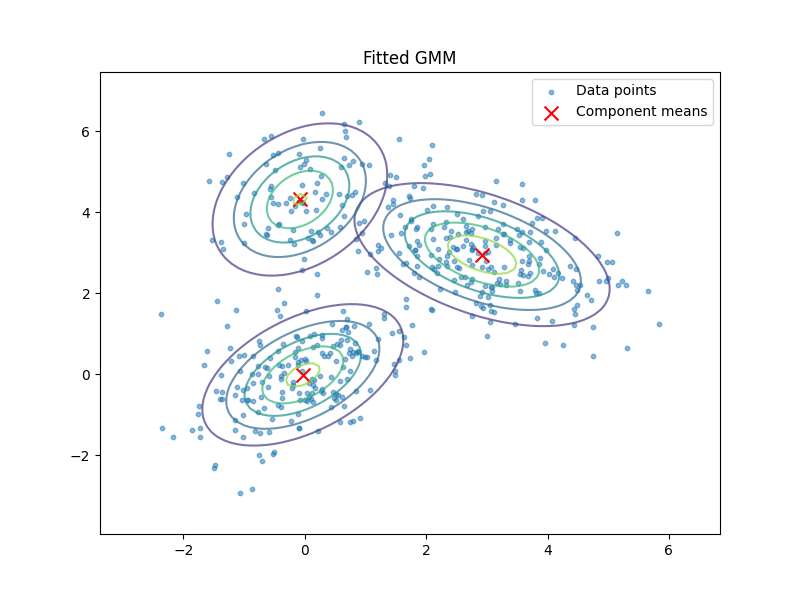
\includegraphics[width=1\textwidth]{fitted GMM visual.png}
% \caption{Fitted Gaussian Mixture Model Visualization}
\label{fig:gmm_visual}
\end{figure}

\clearpage

\section*{Problem 10: Hidden Markov Model}
HMM is a probabilistic model used to describe systesm that undergo changes over time in a way that depends on hidden states. In the problem given the patient condition is
hidden thatis the viral and bacteria but we can observe the temperature that is High or nomral tha tgives us the inderect evidence about the condition.

\subsection*{Key Components of an HMM}

\begin{enumerate}
    \item \textbf{Hidden States (\(\mathcal{S}\))}:  
    These are the actual states of the system, which we cannot directly observe.  
    For this problem, the two hidden states are:  
    \begin{itemize}
        \item \textbf{"Viral" (V)}: Patient has a viral infection  
        \item \textbf{"Bacterial" (B)}: Patient has a bacterial infection  
    \end{itemize}

    \item \textbf{Observations (\(\mathcal{O}\))}:  
    These are the observable variables dependent on the hidden states.  
    For this problem, the observations are the patient's \textbf{temperature}, which can be:
    \begin{itemize}
        \item \textbf{"Normal" (N)}: Patient's temperature is normal.
        \item \textbf{"High" (H)}: Patient has a high temperature.
    \end{itemize}

    \item \textbf{Initial Probabilities (\(\pi\))}:  
    This represents the probability of the patient being in each state at \textbf{time \( t = 0 \)} (Day 1).  
    \[
    \pi(V) = 0.7, \quad \pi(B) = 0.3
    \]

    \item \textbf{Transition Probabilities (\(A\))}:  
    These represent the probability of transitioning from one state to another between consecutive time steps.  
    \[
    A = 
    \begin{bmatrix}
    P(V \to V) & P(V \to B) \\
    P(B \to V) & P(B \to B)
    \end{bmatrix}
    =
    \begin{bmatrix}
    0.8 & 0.2 \\
    0.4 & 0.6
    \end{bmatrix}
    \]

    \item \textbf{Emission Probabilities (\(B\))}:  
    These represent the probability of observing a symptom \textbf{given the hidden state}.  
    \[
    B =
    \begin{bmatrix}
    P(N|V) & P(H|V) \\
    P(N|B) & P(H|B)
    \end{bmatrix}
    =
    \begin{bmatrix}
    0.6 & 0.4 \\
    0.3 & 0.7
    \end{bmatrix}
    \]
\end{enumerate}

We need to \textbf{compute the probability} of observing the sequence \textbf{(Normal, High, High)} over three days using two algorithms:
\begin{enumerate}
    \item \textbf{Forward Algorithm (\(\alpha\))}.
    \item \textbf{Backward Algorithm (\(\beta\))}.
\end{enumerate}

\subsection*{1. Forward Algorithm (\(\alpha\))}
The \textbf{Forward Algorithm} is used to compute the probability of an observation sequence \textbf{efficiently} using \textbf{dynamic programming}.

The forward probability \(\alpha_t(s)\) represents the probability of being in state \( s \) at time \( t \) given the observed sequence up to \( t \).

\begin{enumerate}
    \item \textbf{Initialization (\( t = 0 \))}:  
    \[
    \alpha_0(s) = \pi(s) B(s, O_0)
    \]

    \item \textbf{Recursion (\( t > 0 \))}:  
    \[
    \alpha_t(s) = \sum_{s'} \alpha_{t-1}(s') A(s', s) B(s, O_t)
    \]

    \item \textbf{Termination}:  
    \[
    P(O) = \sum_{s} \alpha_T(s)
    \]
\end{enumerate}

\subsection*{2. Backward Algorithm (\(\beta\))}
The \textbf{Backward Algorithm} is similar but works in \textbf{reverse order}, computing the probability of the remaining observations given a state at time \( t \).

\begin{enumerate}
    \item \textbf{Initialization (\( t = T \))}:  
    \[
    \beta_T(s) = 1
    \]

    \item \textbf{Recursion (\( t < T \))}:  
    \[
    \beta_t(s) = \sum_{s'} A(s, s') B(s', O_{t+1}) \beta_{t+1}(s')
    \]

    \item \textbf{Compute \( P(O) \) using \( \beta \)}:  
    \[
    P(O) = \sum_{s} \pi(s) B(s, O_0) \beta_0(s)
    \]
\end{enumerate}

\subsection*{Generally}
\begin{itemize}
    \item \textbf{Forward algorithm} computes the probability \textbf{incrementally}.
    \item \textbf{Backward algorithm} computes the probability \textbf{from the end}.
    \item Both methods should \textbf{yield the same result}.
\end{itemize}

\subsection*{Steps for Implementation}
\begin{enumerate}
    \item Define the transition matrix \( A \) and emission matrix \( B \).
    \item Implement the forward algorithm step-by-step.
    \item Implement the backward algorithm step-by-step.
    \item Verify that both methods produce the same probability.
    \item Print intermediate steps for debugging.
\end{enumerate}

\subsubsection*{How are the probabilities stored and how are they used for infererence? Please Explain}
The probabilities are stored in matrices or tables, such as the transition matrix \(A\), 
emission matrix \(B\), and initial probabilities \(\pi\). These matrices are used for inference 
by applying Forward and Backward algorithms to compute the likelihood of observation sequences or
 to determine the most probable sequence of hidden states.

From the above explanation how i came up with the solution we concluded that forward aligorithm computes probability incrementally
and the backward aligorithm from the end.

These probabilities enables us to perform the following:
1. Predicting the likelihood of a sequence of observations.
2. Decoding the most probable sequence of hidden states using the Viterbi algorithm.
3. Estimating model parameters using the Baum-Welch algorithm.

\subsubsection*{The implimentation output}
\textbf{Forward Algorithm Table}
\begin{table}[H]
\centering
\begin{tabular}{|c|c|c|}
\hline
\textbf{Time (t)} & \textbf{Viral (\(\alpha[\text{Viral}][t]\))} & \textbf{Bacterial (\(\alpha[\text{Bacterial}][t]\))} \\ \hline
0 (Normal)        & 0.4200                                      & 0.0900                                           \\ \hline
1 (High)          & 0.1488                                      & 0.0966                                           \\ \hline
2 (High)          & 0.0631                                      & 0.0614                                           \\ \hline
\end{tabular}
% \caption{Forward Algorithm Table (\(\alpha[\text{state}][\text{time}]\))}
\end{table}

\noindent
\textbf{Probability of the observation sequence (N, H, H):} 0.124476

\textbf{Backward Algorithm Table}
\begin{table}[H]
\centering
\begin{tabular}{|c|c|c|}
\hline
\textbf{Time (t)} & \textbf{Viral (\(\beta[\text{Viral}][t]\))} & \textbf{Bacterial (\(\beta[\text{Bacterial}][t]\))} \\ \hline
2 (High)          & 1.0000                                      & 1.0000                                           \\ \hline
1 (High)          & 0.4600                                      & 0.5800                                           \\ \hline
0 (Normal)        & 0.2284                                      & 0.3172                                           \\ \hline
\end{tabular}
% \caption*{Backward Algorithm Table (\(\beta[\text{state}][\text{time}]\))}
\end{table}

\noindent
\textbf{Backward Probability:} 0.124476



\clearpage

\section*{Problem 11: Maximum A Posteriori estimation}
\subsection*{Maths of MAP estimation}
MAPis away of estimating the probablity distribution by incoprating the prior beliefs, by that it means given a set of observed data d,
MAP estimation chooses the class C that maximizes the Posteriori probablity.
\[
P(C|d) = \frac{P(d|C)P(C)}{P(d)}
\]
\begin{itemize}
    \item \(P(C|d)\) - is the posterior probability of class \(C\) given document \(d\).
    \item \(P(d|C)\) - is the likelihood of document \(d\) occuring given class \(C\).
    \item \(P(C)\) - is the prior probability of class \(C\).
    \item \(P(d)\) - is the evidence or the probability of document \(d\).
\end{itemize}
Since \(P(d)\) is the same across all the classes we igone it and compute:
\[
\argmax_C P(d|C)P(C)
\]
Therefore we need to calculate:
\begin{itemize}
    \item \(P(C)\) - prior probablity of each class
    \item \(P(d|C)\) - The likelihood of the document given the class
\end{itemize}

\subsection*{MAP and Niave Bayes relationship}
This task is similar to NB classifiere since it assumes:
\begin{itemize}
    \item \textbf{Conditional Independence} the words in the document are Independent given the class.
    \item \textbf{MultinomialModel} the probablity of the document is the product of indivisdual word probablities.
\end{itemize}
Applying the Naive Bayes (NB) assumption, the likelihood \(P(d|C)\) is given by:
\[
P(d|C) = \prod_{i=1}^{n} P(w_i|C)
\]
where:
\begin{itemize}
    \item \(w_i\) represents the \(i\)-th word in the document \(d\),
    \item \(P(w_i|C)\) is the probability of word \(w_i\) given class \(C\),
    \item \(n\) is the total number of words in the document.
\end{itemize}
Takind the log to avaoid underflow of issues:
\[
\log P(d|C) = \sum_{i=1}^{n} \log P(w_i|C)
\]
Thus, the MAP estimation becomes:
\[
\argmax_C \left( \log P(C) + \sum_{i=1}^{n} \log P(w_i|C) \right)
\]

\subsection*{Multinomial Distribution and Text classification}
\begin{itemize}
    \item document represents a bag o f words i.e word frequencies
    \item probability of a document given the class is the product of word occuracne probablity
    \item Each word's probability in a class is estimated as:
    \[
    P(w_i|C) = \frac{\text{count}(w_i, C) + \alpha}{\text{count}(C) + \alpha \cdot V}
    \]
    where:
    \begin{itemize}
        \item \(\text{count}(w_i, C)\) is the number of times word \(w_i\) appears in documents of class \(C\),
        \item \(\text{count}(C)\) is the total number of words in documents of class \(C\),
        \item \(\alpha\) is the smoothing parameter (Laplace smoothing),
        \item \(V\) is the size of the vocabulary.
    \end{itemize}
\end{itemize}

\subsection*{Implimentation approach}
\begin{enumerate}
    \item \textbf{Preprocessing Text Data}
    \begin{itemize}
        \item convert text to lowercase
        \item remove punctuation and stop words
        \item tokenize into words
        \item represent documnt as word count vectors
    \end{itemize}
    \item \textbf{Train the MAP-Based Classifier}
    \begin{itemize}
        \item Compute class priors: \(P(C) = \frac{count of doccs in C}{total docs}\)
        \item Compute word probability for each class using laplace smoothing
    \end{itemize}
    \item \textbf{Predict the new document's class}
    \begin{itemize}
        \item Compute the posterior probability for each class using:
        \[
        \log P(C|d) = \log P(C) + \sum_{i=1}^{n} \log P(w_i|C)
        \]
        \item Select the class \(C\) with the highest posterior probability:
        \[
        C_{\text{predicted}} = \argmax_C \left( \log P(C) + \sum_{i=1}^{n} \log P(w_i|C) \right)
        \]
    \end{itemize}
    \textbf{The solution is in MAP.py script}
\end{enumerate}


\end{document}